\documentclass[11pt, letterpaper, openany, oneside]{article}

\usepackage[utf8]{inputenc}
\usepackage{amsmath}
\usepackage{amsfonts}
\usepackage{amssymb}
\usepackage{graphicx}
\usepackage{sectsty}
\usepackage{titlesec}
\usepackage{color}
\usepackage{hyperref}
\usepackage{t1enc}
\usepackage{paralist}
\usepackage[hungarian]{babel}

\title{\textbf{NAR Morsecode Adó/Vevő}}
\author{\LARGE Gáspár Róbert \vspace{4px} \\ K8FD5S}
\date{\today}

\hypersetup{
    colorlinks,
    linktoc=all,
    linkcolor={blue},
    citecolor={blue},
    urlcolor={blue}
}

\begin{document}

\maketitle

\tableofcontents

\section{Schematika}

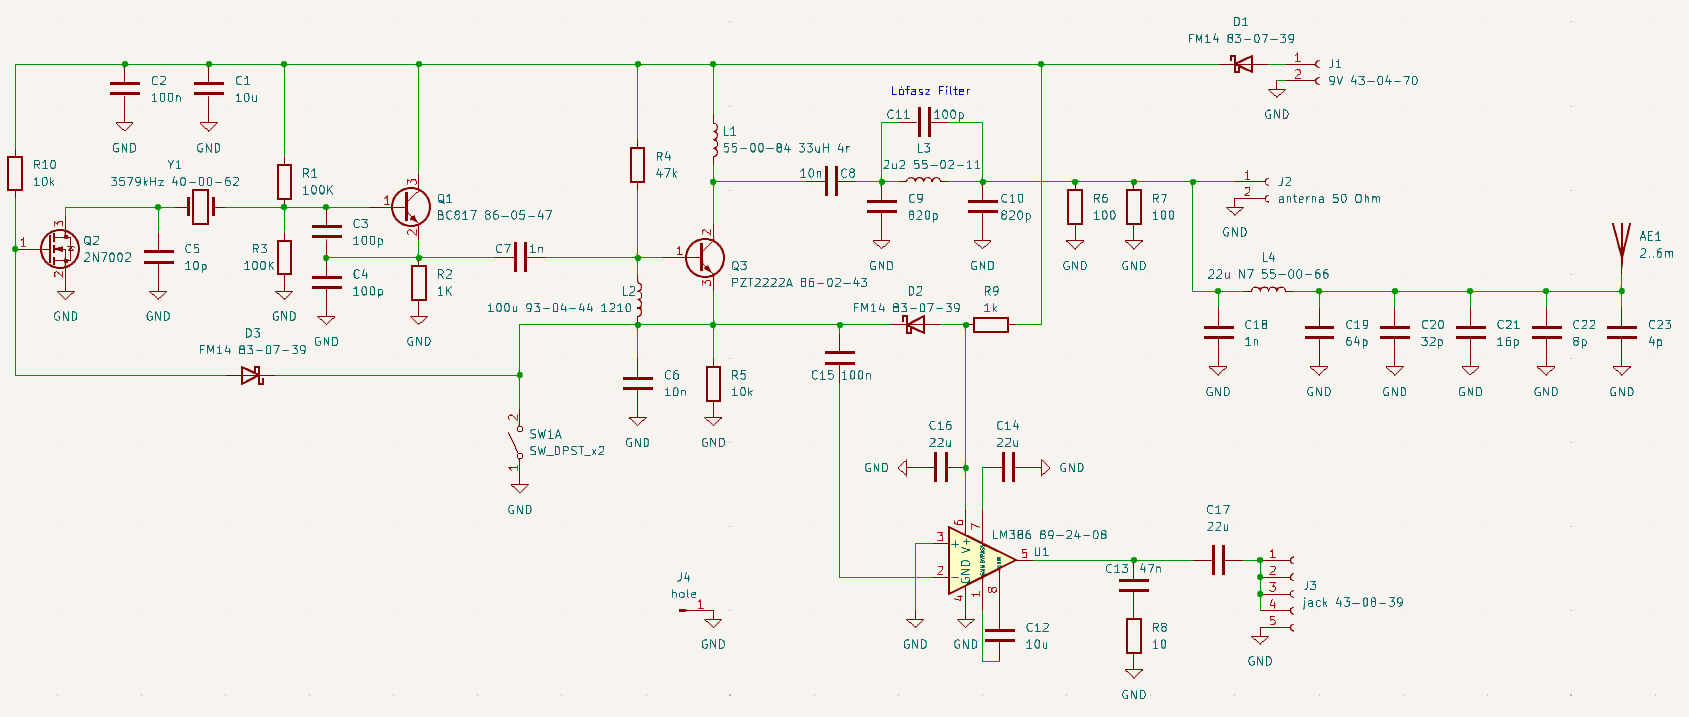
\includegraphics[width=\linewidth]{img/sch.png}

\section{Pcb Elrendezés}

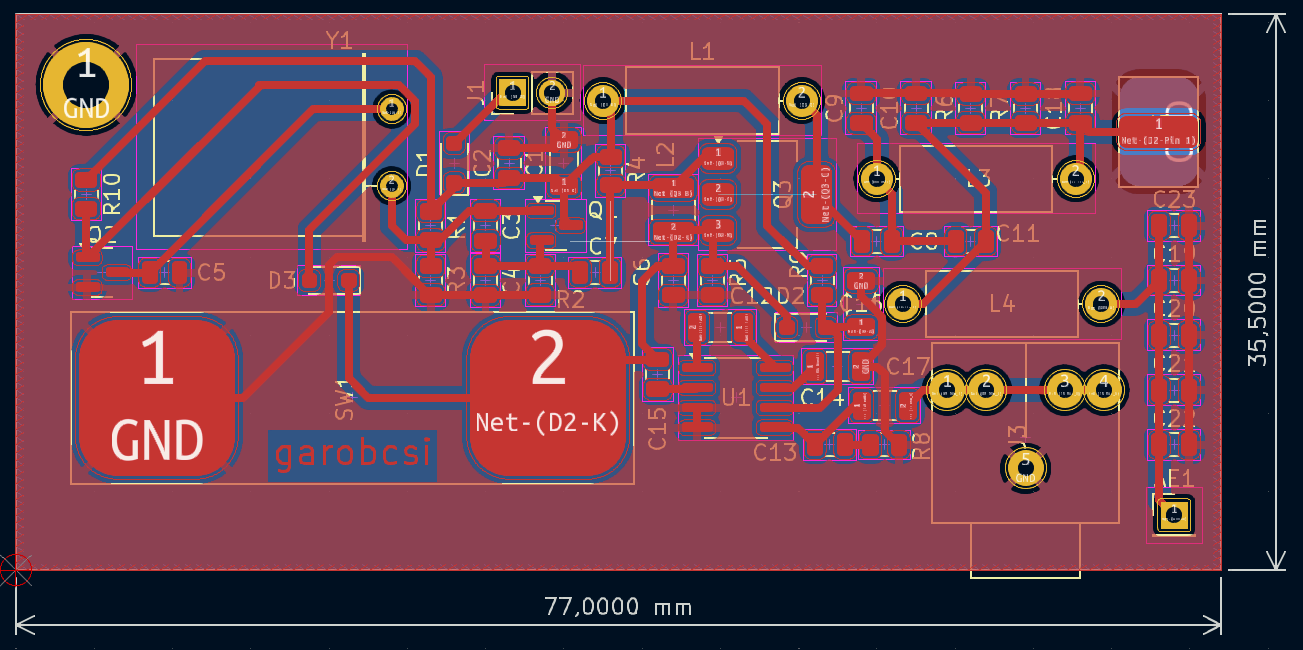
\includegraphics[width=\linewidth]{img/pcb.png}

\section{Pcb Elrendezés 3D}

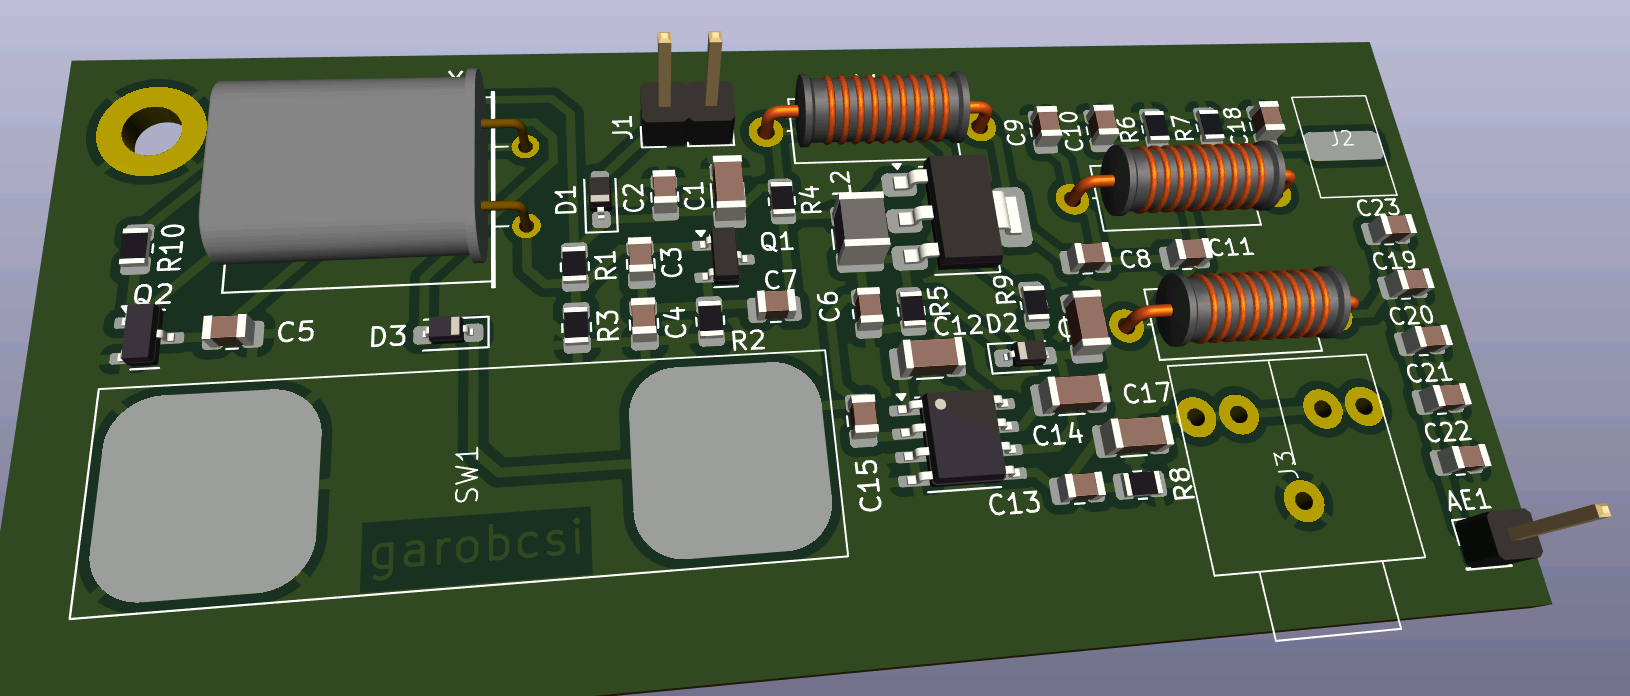
\includegraphics[width=\linewidth]{img/pcb 3d.png}

\section{Elkésztett Pcb}

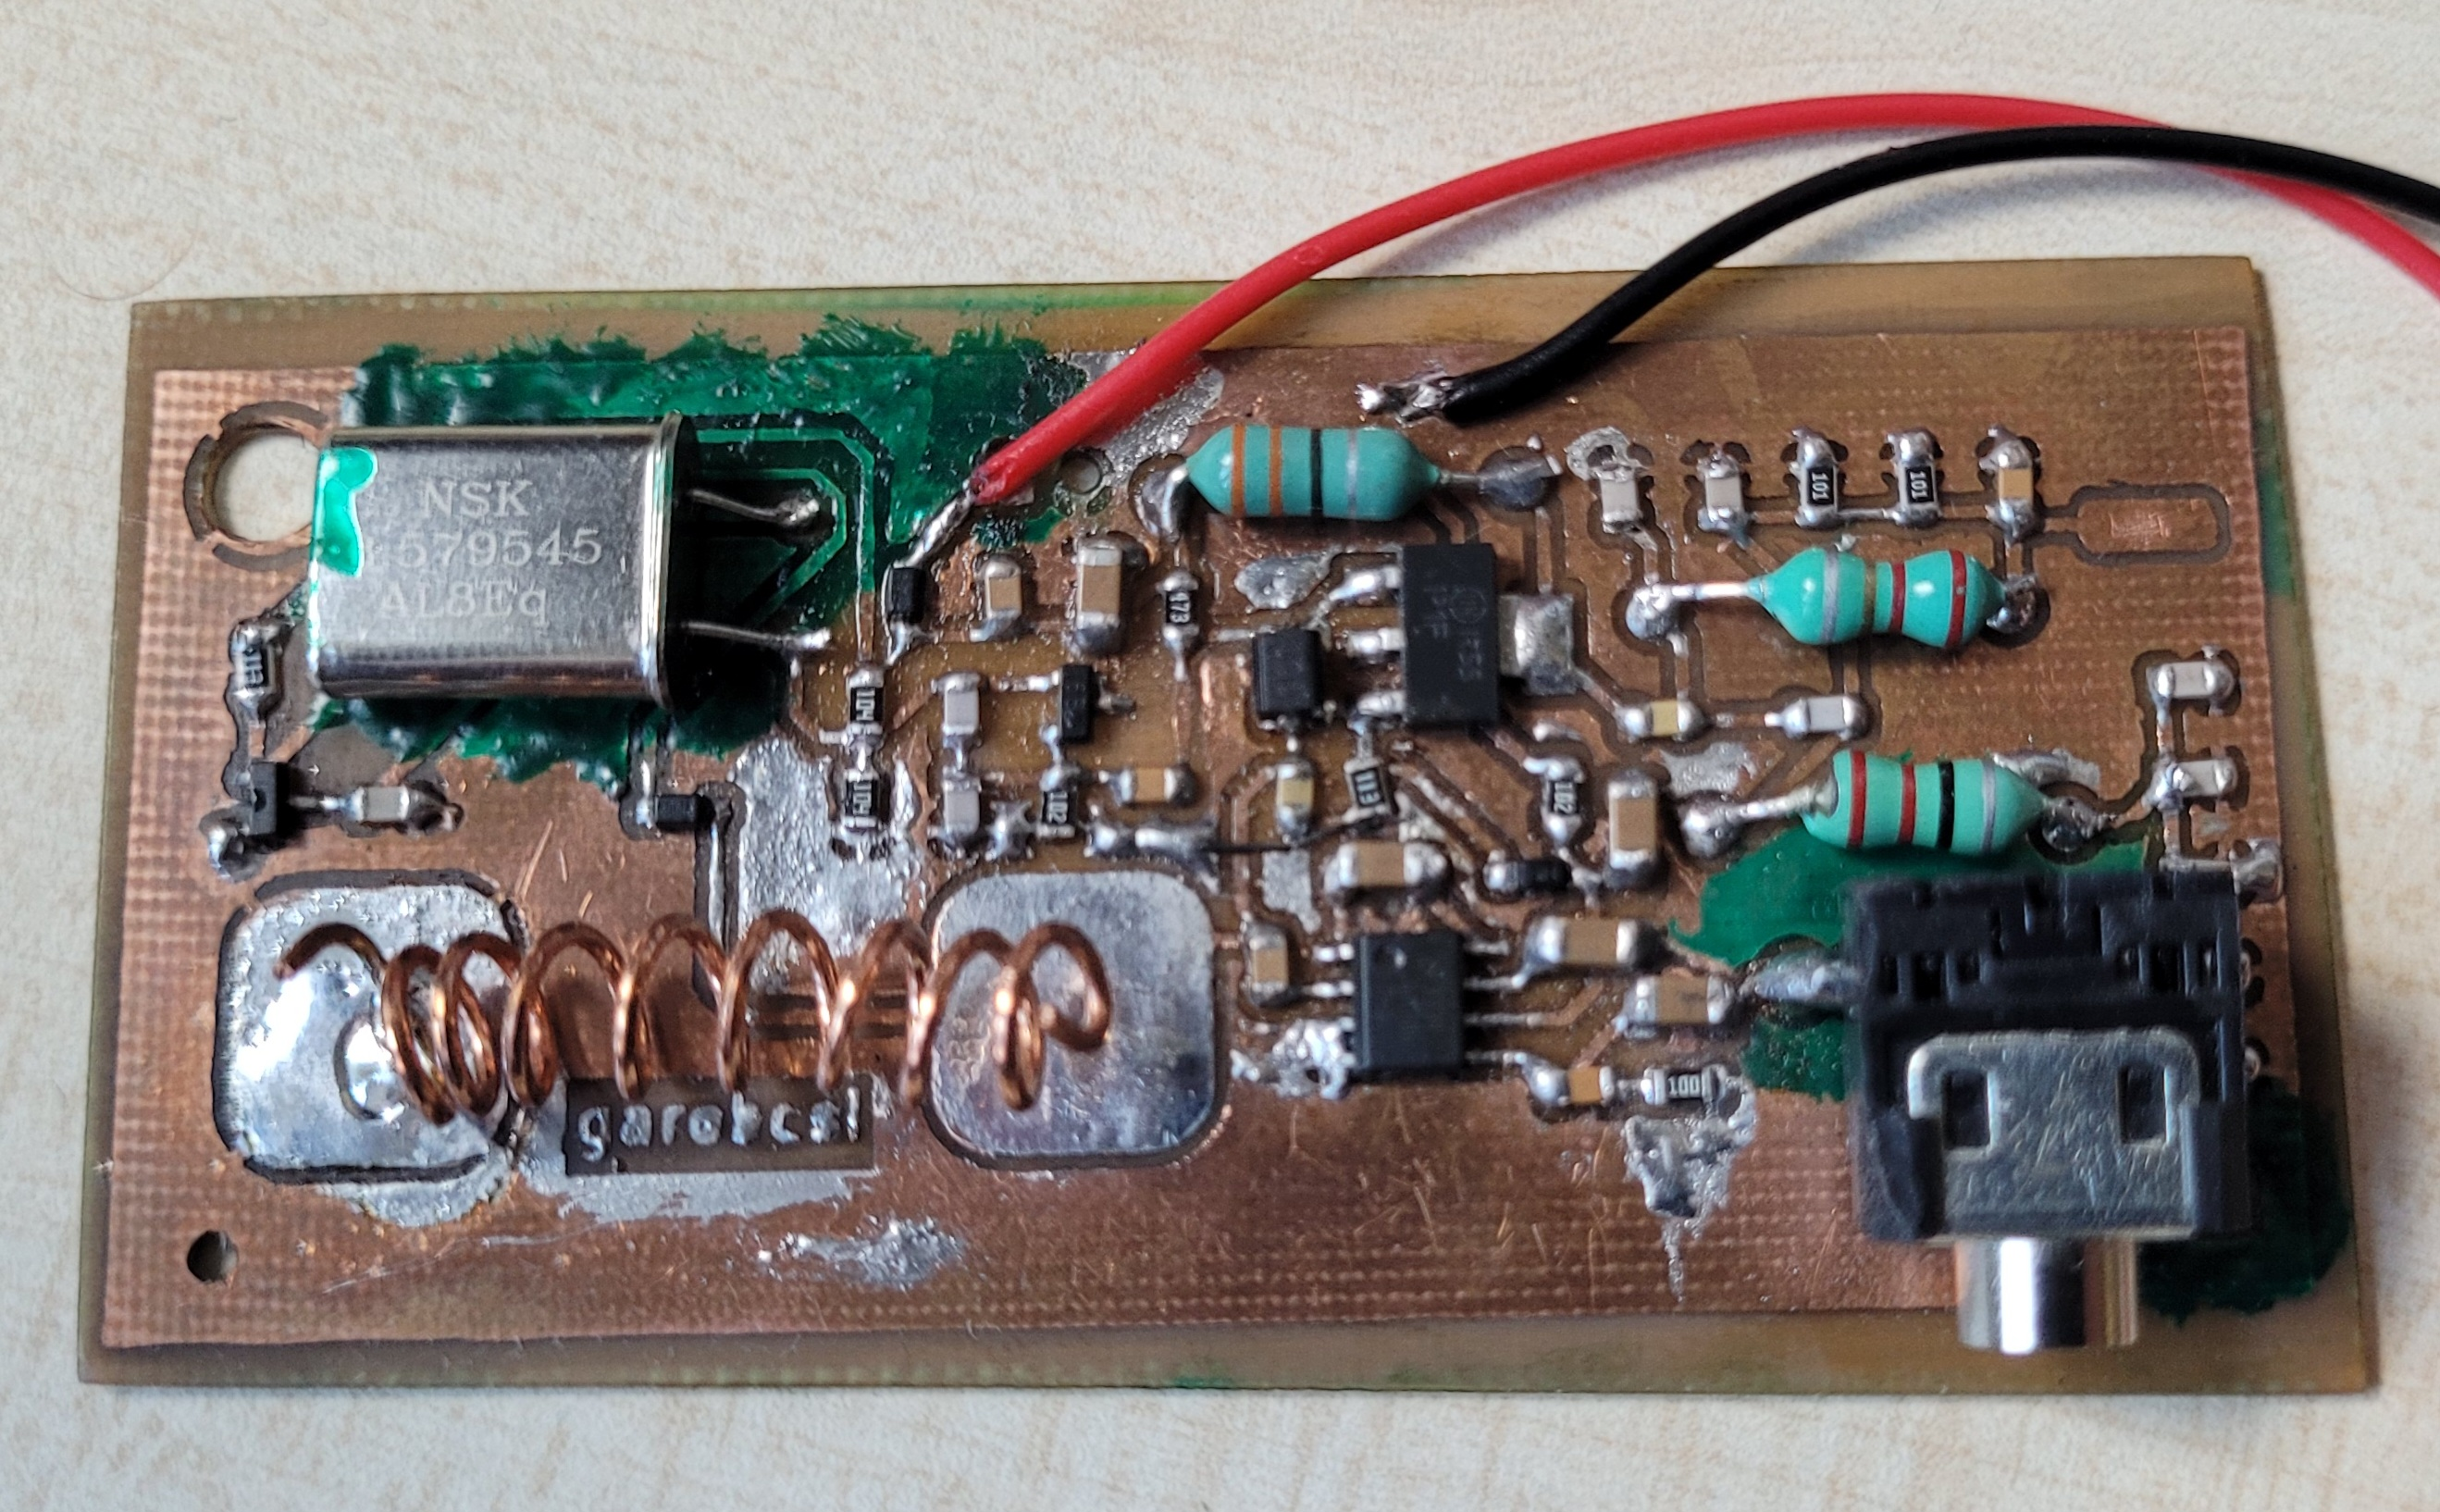
\includegraphics[width=\linewidth]{img/irl.jpg}

\section{Oszcilloszkóp Mérések}

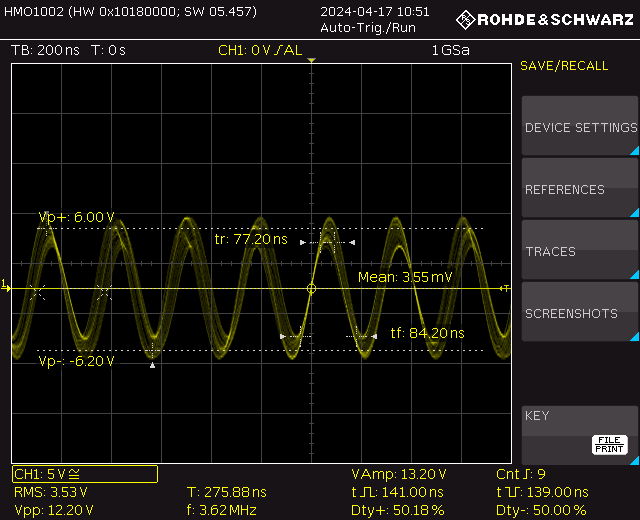
\includegraphics[width=\linewidth]{img/KITTYK01.PNG}
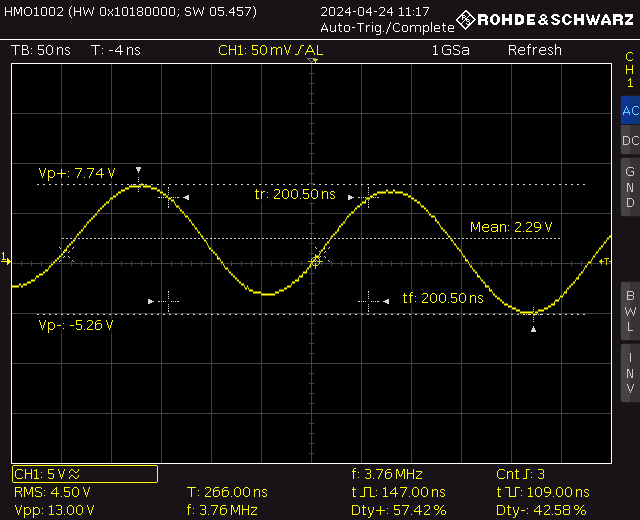
\includegraphics[width=\linewidth]{img/KITTYK02.PNG}
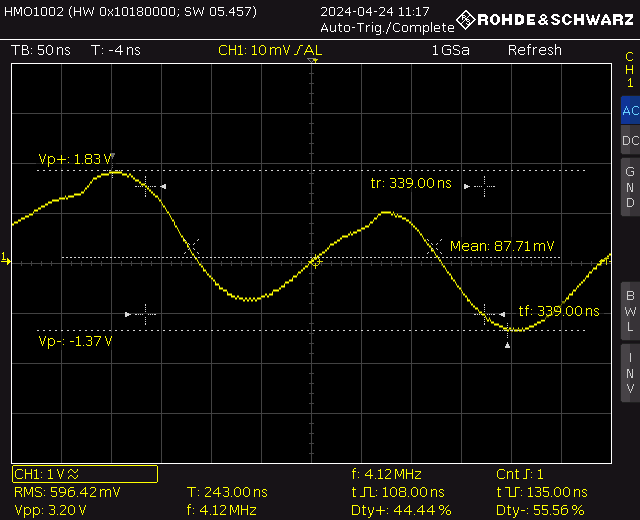
\includegraphics[width=\linewidth]{img/KITTYK03.PNG}
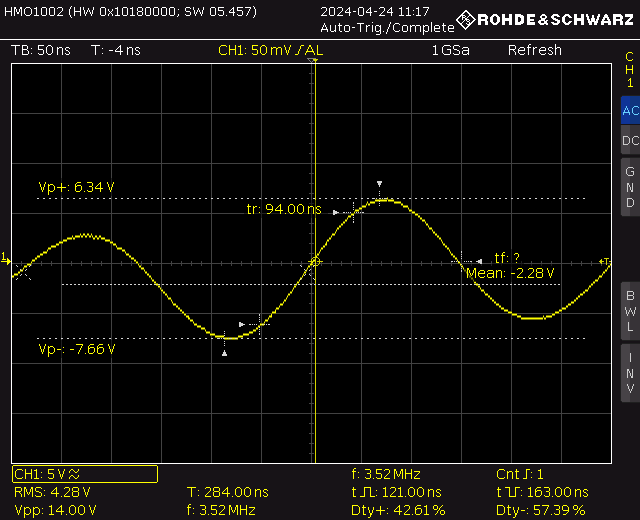
\includegraphics[width=\linewidth]{img/KITTYK04.PNG}

\section{Elem Multiméter Mérés}

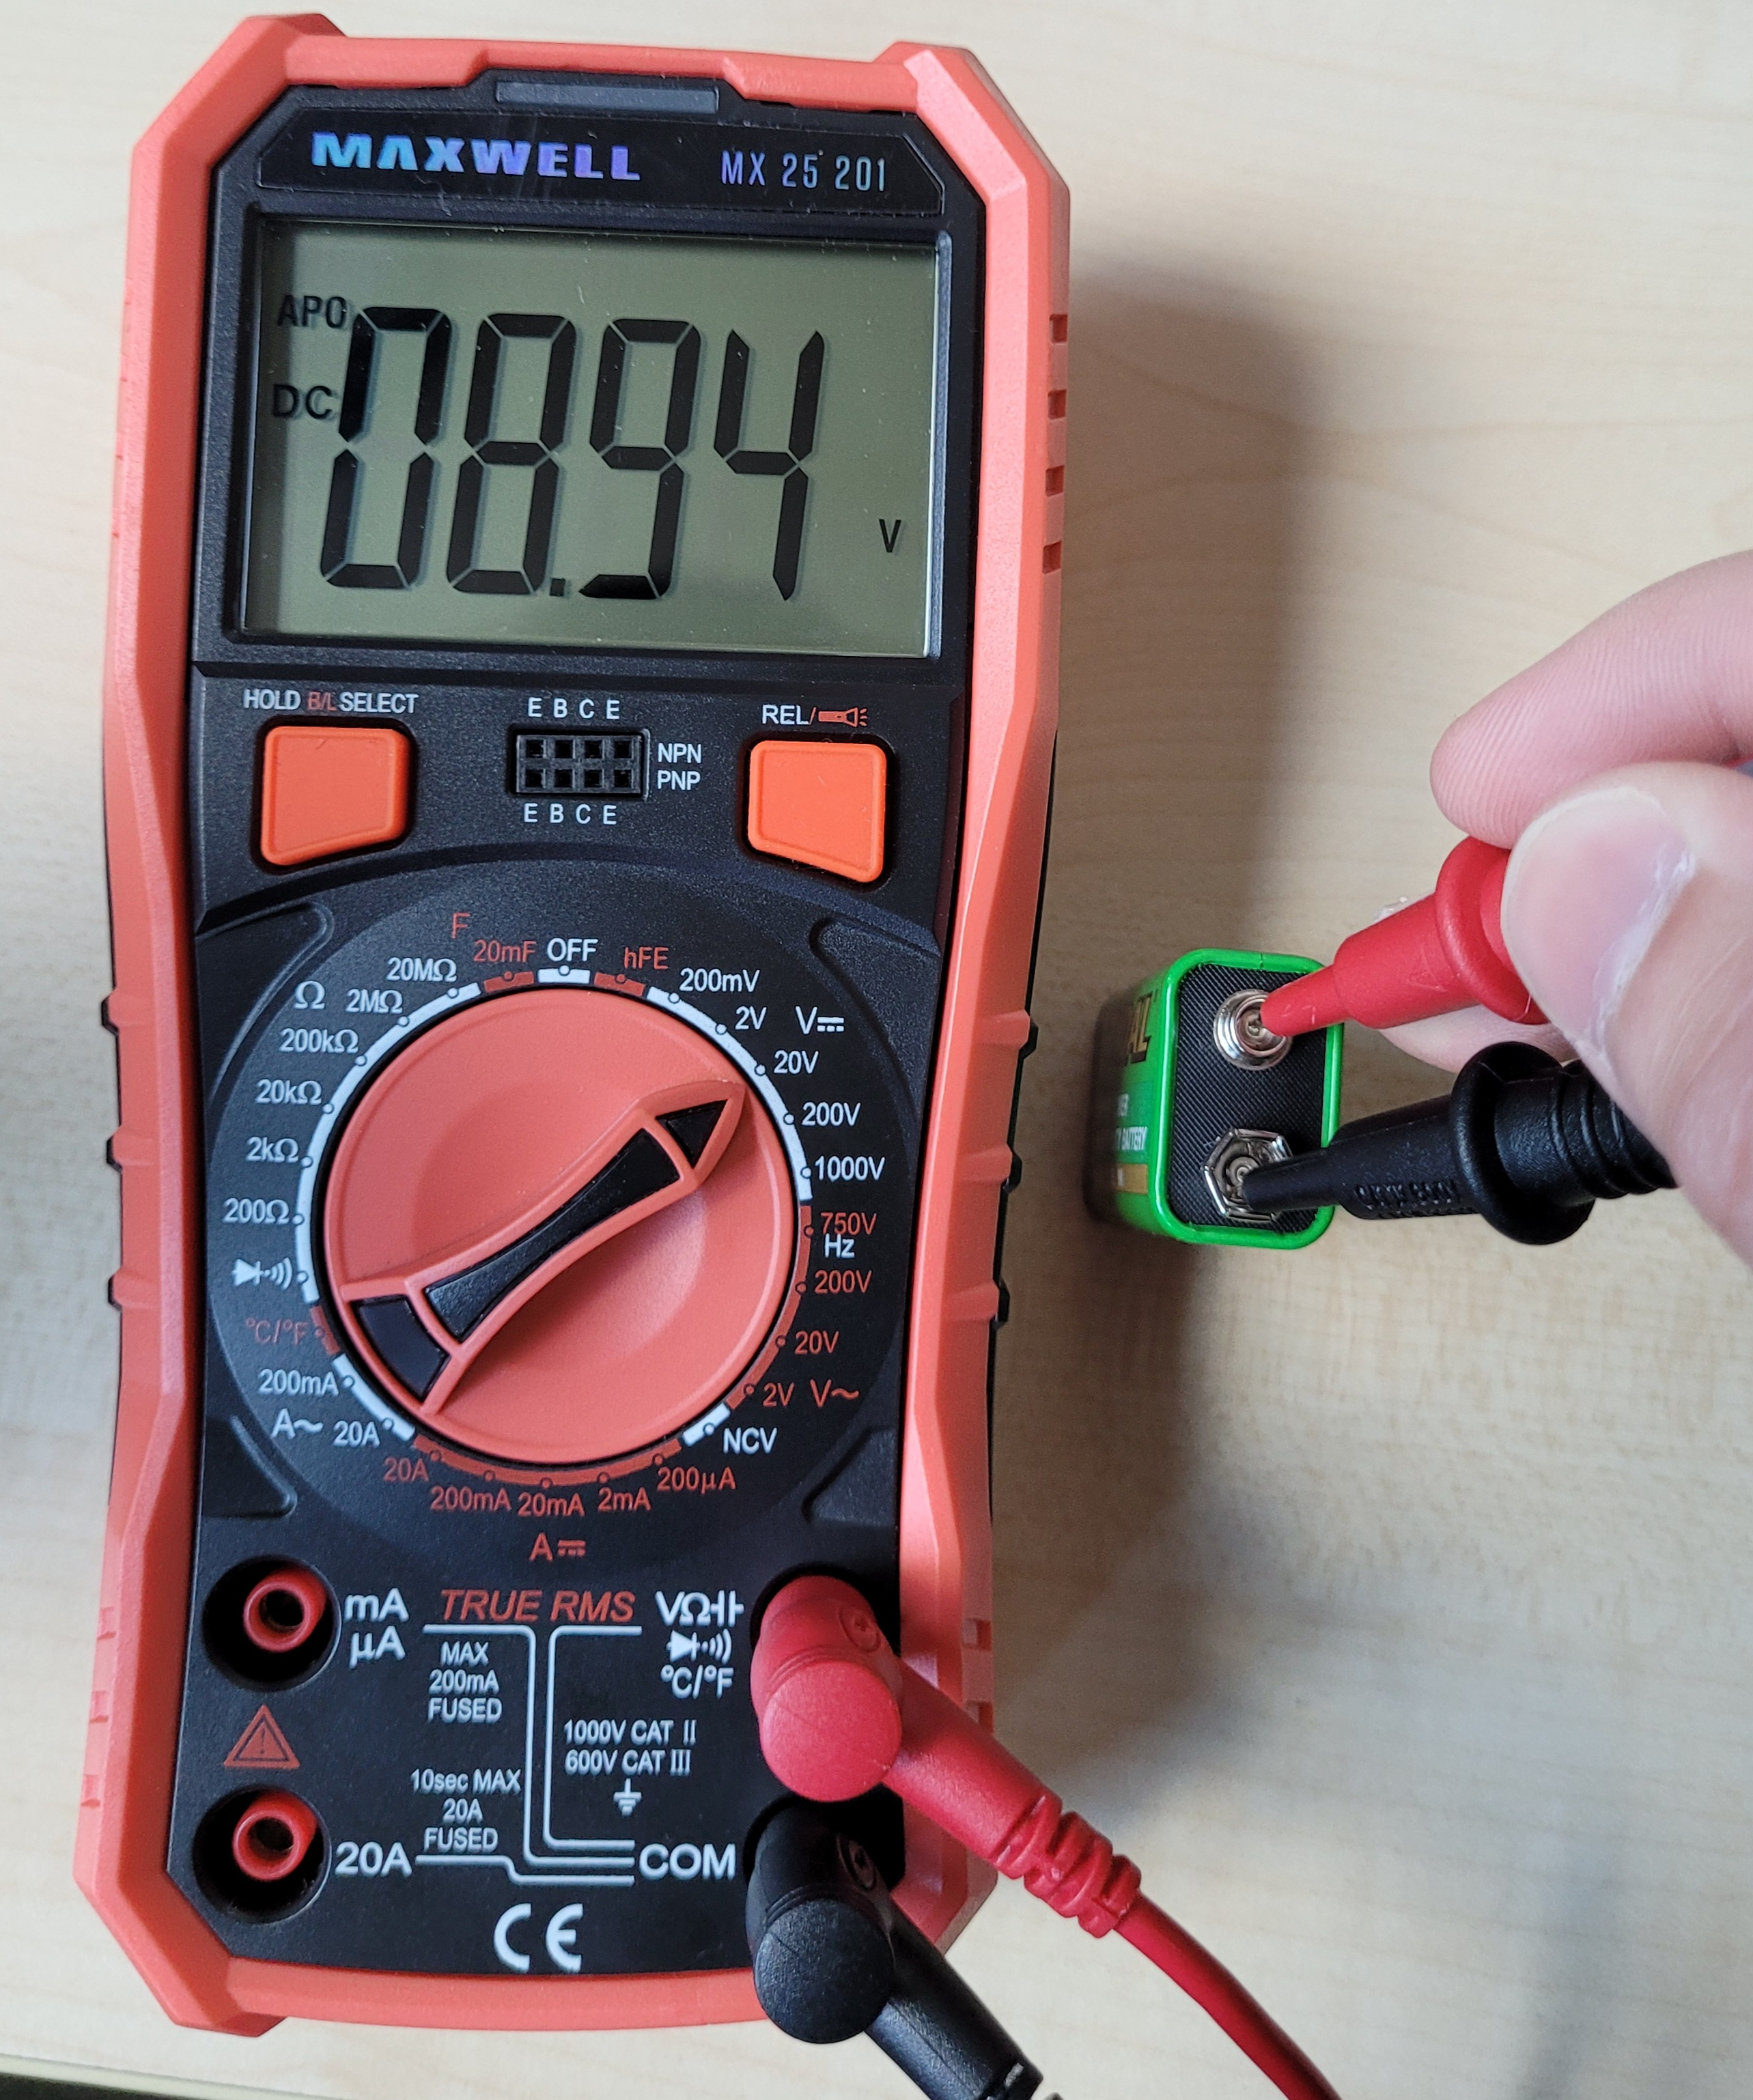
\includegraphics[width=\linewidth]{img/bat.jpg}


\end{document}